\documentclass[a4paper, 12pt]{article}
\usepackage{a4wide}
\usepackage {amsmath}
\usepackage{amssymb}
\usepackage {graphicx}
\usepackage[utf8]{inputenc} 
\usepackage[francais]{babel}
\usepackage{fancyhdr}
\usepackage{setspace}
\usepackage{fancyhdr}
\usepackage{lastpage}
\usepackage{extramarks}
\usepackage{chngpage}
\usepackage{soul}
\usepackage{algorithmicx} 
\usepackage{algpseudocode} 
\usepackage{multicol}
\usepackage[usenames,dvipsnames]{color}
\usepackage{graphicx,float,wrapfig}
\usepackage{ifthen}
\usepackage{listings}
\usepackage{courier}
\usepackage{esint}
\usepackage{bbm}
\usepackage{graphics}
\usepackage{graphicx}
\usepackage{subfig}
\usepackage{epsfig}
\usepackage{pgf,tikz}
\usetikzlibrary{arrows}
\usepackage{braket}
\usepackage{MnSymbol,wasysym}
\usepackage{marvosym}
\usepackage{dsfont}
\usepackage{stmaryrd}
\usepackage{wrapfig}
\usepackage{enumitem}

\lhead{} 
\chead{} 
\rhead{\bfseries DS de Conduction} 
\lfoot{J.C. Toussaint}
%\cfoot{J.C. Toussaint} 
%\rfoot{\thepage}

% This is the color used for MATLAB comments below
\definecolor{MyDarkGreen}{rgb}{0.0,0.4,0.0}

% For faster processing, load Matlab syntax for listings
\lstloadlanguages{Matlab}%
\lstset{language=Matlab,                        % Use MATLAB
        frame=single,                           % Single frame around code
        basicstyle=\small\ttfamily,             % Use small true type font
        keywordstyle=[1]\color{Blue}\bf,        % MATLAB functions bold and blue
        keywordstyle=[2]\color{Purple},         % MATLAB function arguments purple
        keywordstyle=[3]\color{Blue}\underbar,  % User functions underlined and blue
        identifierstyle=,                       % Nothing special about identifiers
                                                % Comments small dark green courier
        commentstyle=\usefont{T1}{pcr}{m}{sl}\color{MyDarkGreen}\small,
        stringstyle=\color{Purple},             % Strings are purple
        showstringspaces=false,                 % Don't put marks in string spaces
        tabsize=5,                              % 5 spaces per tab
        %
        %%% Put standard MATLAB functions not included in the default
        %%% language here
        morekeywords={xlim,ylim,var,alpha,factorial,poissrnd,normpdf,normcdf},
        %
        %%% Put MATLAB function parameters here
        morekeywords=[2]{on, off, interp},
        %
        %%% Put user defined functions here
        morekeywords=[3]{FindESS, homework_example},
        %
        morecomment=[l][\color{Blue}]{...},     % Line continuation (...) like blue comment
        numbers=left,                           % Line numbers on left
        firstnumber=1,                          % Line numbers start with line 1
        numberstyle=\tiny\color{Blue},          % Line numbers are blue
        stepnumber=5                            % Line numbers go in steps of 5
        }

% Includes a MATLAB script.
% The first parameter is the label, which also is the name of the script
%   without the .m.
% The second parameter is the optional caption.
\newcommand{\matlabscript}[2]
  {\begin{itemize}\item[]\lstinputlisting[caption=#2,label=#1]{#1.m}\end{itemize}}

%\newcommand{\grad}[1]{\gv{\nabla} #1} % for gradient
\let\divsymb=\div % rename builtin command \div to \divsymb
%\renewcommand{\div}[1]{\gv{\nabla} \cdot #1} % for divergence

%\newcommand{\grad}[1]{\mathbf{\mathrm{grad}} #1} % for gradient
\newcommand{\grad}{\mathbf{grad\; } } % for gradient
\renewcommand{\div}{\mathrm{div\;}} % for divergence

\newcommand{\curl}[1]{\gv{\nabla} \times #1} % for curl
\let\baraccent=\= % rename builtin command \= to \baraccent

\pagestyle{fancy}

\usepackage{pgf,tikz}
\usepackage{mathrsfs}
\usetikzlibrary{arrows}

\begin{document}

\bibliographystyle{alpha}

\title{DS de Conduction Thermique : durée 2h}

%\author{Quentin Rafhay - Jean-Christophe Toussaint\\
%  Phelma\\
%\texttt{jean-christophe.toussaint@phelma.grenoble-inp.fr}
%}
%\date{\today}
\date{\vspace{-10ex}}
 
\maketitle

 \fbox{\parbox{\textwidth}{
Tout document autorisé. Tout ordinateur et toute calculatrice programmable autorisés.
Téléphone portable interdit. Longue-vue interdite.
}}

\vspace{1cm}

\section{Exercice : étude de la fusion d'une sphère de glace dans un milieu aqueux - 6 points}

%\begin{wrapfigure}{r}{5.5cm}
%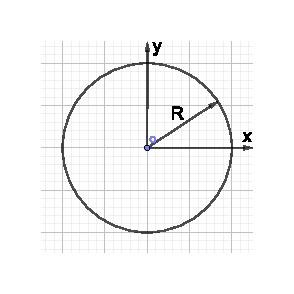
\includegraphics[scale=1.3]{circular_pipe.pdf}
%\caption{Section du canal}
%\label{canal}
%\end{wrapfigure}

On étudie l'évolution du rayon d'une sphère de glace initialement à température $T_s^0 = 0^\circ C$ placée dans de l'eau à température $T_{l}^0 > 0^\circ C$. Le système est placé dans un calorimètre isolé thermiquement.
\vspace{-0.5cm}
\subsubsection*{Paramètres du système et notations}
\begin{itemize}[itemsep=0pt, topsep=2pt, parsep=0pt, partopsep=0pt]
    \item Sphère de glace initiale : température $T_s^0 = T_{mp} = 0^\circ C$, rayon initial $r_0$
    \item Eau environnante : température $T_{l}^0 > 0^\circ C$ (température du fluide loin de la sphère)
    \item Température de fusion/point de fusion : $T_{mp} = 0^\circ C$
    \item Rayon instantané de la sphère : $r_s(t)$
    \item Masse volumique de la glace : $\rho_s$ 
    \item Masse volumique de l'eau : $\rho_l$ 
    \item Chaleur latente de fusion : $h_{sf}$ 
    \item Capacité calorifique de l'eau : $c_{p,l}$
    \item coefficient d'échange thermique à l'interface solide-liquide : $h$
    \item Hypothèse fondamentale : $Bi \ll 1 \Rightarrow$ température uniforme dans la glace à $T_{mp}$
\end{itemize}

Dans le {\color{red} calorimètre parfaitement isolé et fermé}, la masse totale et l'énergie totale du système (glace + eau) se conservent au cours du temps. À l'instant initial, l'énergie totale du système est :
\begin{equation*}
E_{total} = E_{glace}^0 + E_{eau}^0 = 
-{\color{red} m_{s}^0 \cdot h_{sf}} + m_{s}^0 \cdot c_{p,s} \cdot (T_s^0-T_{ref}) + m_{l}^0 \cdot c_{p,l} \cdot (T_{l}^0-T_{ref})
\end{equation*}
Une autre définition en ajoutant la constante ${\color{red} (m_s^0+m_l^0) \cdot h_{sf}}$ est:
\vspace{-0.2cm}
\begin{equation*}
E_{total} = E_{glace}^0 + E_{eau}^0 = 
 m_{s}^0 \cdot c_{p,s} \cdot (T_s^0-T_{ref}) + m_{l}^0 \cdot c_{p,l} \cdot (T_{l}^0-T_{ref})
+{\color{red} m_{l}^0 \cdot h_{sf}}
\end{equation*}
Il est judicieux de prendre ici $T_{ref}=0^\circ C$ et d'exprimer toutes les températures en degrés Celsius.


À l'instant initial, l'énergie totale du système est :
\begin{equation*}
E_{total} = E_{glace}^0 + E_{eau}^0 = 
 -m_{s}^0 \cdot h_{sf} + m_{s}^0 \cdot c_{p,s} \cdot (T_s^0-T_{ref}) + m_{l}^0 \cdot c_{p,l} \cdot (T_{l}^0-T_{ref})
\end{equation*}
avec $T_{ref} = 0^\circ C$.

\begin{enumerate}[itemsep=2pt, topsep=2pt, parsep=0pt, partopsep=2pt]
\item Écrire la conservation de la masse totale pour tout instant $t>0$. En déduire l'expression de $m_{l}(t)$ en fonction de $m_s(t)$, entre autres.
\item Écrire l'énergie totale du système à tout instant $t$. En déduire l'expression de la température de l'eau $T_l(t)$.
\item Écrire l'expression de la masse de la sphère de glace en fonction de son rayon. En déduire l'expression de sa dérivée temporelle.
\item Le transfert de chaleur de l'eau vers la glace s'effectue par convection.  
Toute l'énergie thermique entrant dans la sphère est utilisée pour la fusion :
\[
\dot{Q}_{\text{fusion}} = -h_{sf} \frac{dm_s}{dt}
\]
Vérifier que $\dot{Q}_{\text{fusion}}>0$.
\item En déduire l'expression de la vitesse $\dot{r}_s$ en fonction de $T_l(t)$.
\item Remplacer $T_l(t)$ dans l'expression de $\dot{r}_s$ par la formule obtenue précédemment.
\item Résoudre dans la limite où la masse de liquide est infiniment grande.
\end{enumerate}

\section{Exercice : mur plan avec convection - 6 points}

Considérons un \textit{mur plan} d'épaisseur $2L$. Si l'épaisseur est petite par rapport à la largeur et à la hauteur du mur, il est raisonnable de supposer que la conduction se produit exclusivement dans la direction $x$. 

Le mur est initialement à une température uniforme, $T(x, 0) = T_i$, et est soudainement immergé dans un fluide de température $T_\infty \neq T_i$. Les surfaces placées en $x=\pm L$ échangent de la chaleur
par convection.

Les distributions de température sont obtenues en résolvant l'équation de la chaleur. Puisque les conditions de convection pour les surfaces à $x^* = \pm 1$ sont les mêmes, la distribution de température à tout instant doit être symétrique par rapport au plan médian ($x^* = 0$). 

\begin{enumerate}[itemsep=2pt, topsep=2pt, parsep=0pt, partopsep=2pt]
\item Ecrire l'expression de l'échange convectif en surface en précisant son unité physique.
\item On veut résoudre l'équation de la chaleur dépendante du temps sans terme source, en utilisant deux variables adimensionnelles notées $x^*$, $F\!o$. Préciser leur expression.
\item Expliquer précisément, comment il est possible d'écrire l'équation de la chaleur
\begin{equation}
\frac{\partial^2 T}{\partial x^2} = \frac{1}{\alpha} \frac{\partial T}{\partial t} \quad \text{avec} \quad
\alpha = \frac{k}{\rho c}.
\end{equation}

sous la forme suivante en utilisant les variables adimensionnelles :
\begin{equation}
\frac{\partial^2 \theta^*}{\partial x^{*2}} = \frac{\partial \theta^*}{\partial F\!o}
\end{equation}
Préciser l'expression de $\theta(x^*, F\!o)$ adaptée à ce problème.

\item La solution générale à ce problème est de la forme :
\begin{equation}
\theta^* = \sum_{n=1}^{\infty} \exp(-\zeta_n^2 F\!o) \Big( C_n \cos(\zeta_n x^*) +
D_n \sin(\zeta_n x^*)   \Big)
\end{equation}
Montrer que le coéfficient $D_n$ est nul et que 
$$
C_n = \frac{4 \sin \zeta_n}{2\zeta_n + \sin(2\zeta_n)}.
$$

\item Montrer que les valeurs discrètes de $\zeta_n$ sont les racines positives de l'équation transcendante:
\begin{equation}
\zeta_n \tan \zeta_n = Bi
\end{equation}

\item Proposer deux méthodes pour estimer les premières valeurs $\zeta_n$.
\item Identifier le temps caractérique le plus grand et donner son expression.
\item Tracer les allures de $\theta^*(x^*, F\!o)$ à différents instants pour $Bi \ll 1$ d'une part et 
pour $Bi \gg1$ d'autre part.

\end{enumerate}

\section{Exercice : passages cannelés - 8 points}

% ici on force le wrap sur 8 lignes seulement
\begin{wrapfigure}[12]{r}[0pt]{6cm}
  \centering
  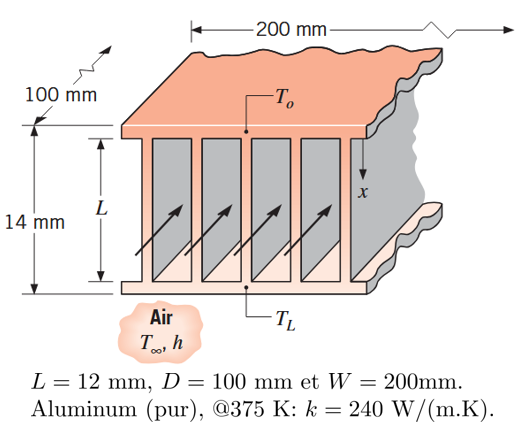
\includegraphics[width=6cm]{passages_canneles.png}
  \caption{Passages cannelés}
  \label{canal}
\end{wrapfigure}

Les passages cannelés sont fréquemment formés entre des plaques parallèles pour améliorer le transfert thermique par convection dans les noyaux d'échangeurs thermiques compacts. Une application importante se trouve dans le refroidissement d'équipements électroniques, où une ou plusieurs piles refroidies par air sont placées entre des composants électriques dissipant de la chaleur. Considérons une pile unique d'ailettes rectangulaires de longueur $L$ et d'épaisseur $t$, avec des conditions de convection correspondant à $h$ et $T_{\infty}$. \\

\noindent 
\begin{enumerate}[itemsep=2pt, topsep=2pt, parsep=0pt, partopsep=2pt]
\item Obtenez les expressions des taux de transfert (=flux) thermique des ailettes, $q^x _{f,o}$ et $q^x_{f,L}$, en fonction des températures de base, $T_o$ et $T_L$.\\
{\it Indication} : résoudre l'équation de l'ailette en stationnaire en fixant les températures $T_o$ et $T_L$
en définissant clairement l'expression de $m$.

\item Dans une application spécifique, une pile de $W=200$ mm de large et $D=100$ mm de profondeur contient $N_f=50$ ailettes, chacune de longueur $L = 12$ mm. L'ensemble de la pile est fait d'aluminium, qui fait partout 1 mm d'épaisseur. Si les limitations de température associées aux composants électriques joints aux plaques opposées dictent des températures maximales admissibles de plaques de $T_o = 400$ K et $T_L = 350$ K, quelles sont les dissipations de puissance maximales correspondantes si $h = 150$ W/(m$^2 \cdot$ K) et $T_{\infty} = 300$ K ?

%{\it Indication} : en haut (resp. bas), les dissipations de puissance maximales sont la somme des flux \\ de conduction au sommet des ailettes et des flux de convection sur la face \\horizontale en contact avec l'air.

\end{enumerate}

\end{document}

